%%%%%%%%%%%%%%%%%%%%%%%%%%%%%%%%%%%%%%%%%%%%%%%%%%%%%%%%%%%%%%%%%
%%%%%%%%%%%%%%%%%%%%%%%%%%%%%%%%%%%%%%%%%%%%%%%%%%%%%%%%%%%%%%%%%
\chapter{Trial design model}
\label{sec:CTS}
\label{maths:epoch-defn}

%%%%%%%%%%%%%%%%%%%%%%%%%%%%%%%%%%%%%%%%%%%%%%%%%%%%%%%%%%%%%%%%%
\section{Introduction}

Until now the common practice was to encode the trial design in experimental data files. This is easily illustrated in the estimation case, where parts of the model, e.g. the structural model and the parameters are explicitly encoded in the model file while the other, design related, parts are encoded in the data file. It has the advantage that a software tool processes the data file and associate it with model variables and recognise all characteristics of a study, such as subject-specific measurement time points and values, covariates, variability levels etc. However it has also clear disadvantages because even for simulation purposes some tools utilise data files to encode the design structure. To change the design only in a detail means to change the data file, an error prone and time consuming work. This is clearly not an ideal situation and PharmML addresses this issue.


%%%%%%%%%%%%%%%%%%%%%%%%%%%%%%%%%%%%%%%%%%%%%%%%%%%%%%%%%%%%%%%%%
\section{Trial Design}

Clinical trials are carefully structured and can vary considerably in
their complexity. Typically, a trial will be structured into one or
more groups with each group subject to one or more treatment regimens
and observation protocols. Each group is then allocated individuals
from a population of subjects who have been screened for their
suitability to participate in the trial. In \pharmml we describe the structure and population a trial
explicitly in a dedicated section. This differs from some other
approaches, bit we feel it makes the clinical trial much clearer to
document and easier to encode computationally. 
%More information can be found in chapter~\ref{sec:CTS}).

 Typically in tools such as NONMEM and MONOLIX, the trial design is
 encoded within a tabular data-file. This file contains the dosing
 information, covariates and the experimental observations of each
 individual in the trial. In addition the definition of the structure
 of the clinical trial is also embedded in this table too. Clearly the
 data-file contains a lot of redundant information.
 
 In \pharmml we separate this information into the following three
 classes\footnote{It is interesting to note that the developers of
   PharML had a similar insight and organised data in a similar
   way\cite{NLMEcons:2008}.}:
 %
 \begin{description}
 \item[Population] The attributes of the individuals in the study: the
   population in the population model. Each individual has a weight,
   an age, a gender and numerous other properties that may or may not
   be modelled as covariates in a given model. In addition, these
   properties may change over time.
 \item[Dosing] When and how a drug or drugs are administered to the
   individuals in the trial.
 \item[Measurements] These are the observations taken from each
   individual and specific times during the study. Such measurements
   provide the objective data used during parameter estimation and are
   typically the outputs calculated during a simulation.
 \end{description}
 %
 By separating out these classes of information you can see that the
 information we need to define the clinical trial is as follows:
 %
 \begin{description}
 \item[Trial Structure] The organisation of the trial, how the subjects
   are grouped into different treatment groups and what the dosing
   regiment is within these treatment groups.
 \item[Population] As above, the properties specific to the individual,
   including those that vary over time.
 \item[Individual Dosing] This is related to the treatment regimens
   described in the trial structure, but describes the dosing of each
   subject in the study.
 \end{description}
 %
 The measurement data is then used exclusively for estimation.

%%%%%%%%%%%%%%%%%%%%%%%%%%%%%%%%%%%%%%%%%%%%%%%%%%%%%%%%%%%%%%%%%
\subsection{Structure}
\label{subsec:TrialStructure}

  To define the Trial Structure we have reused, almost verbatim, the
 CDISC Study Design Model \cite{CDISC:2011a}, which is an
 XML representation of a clinical trial. Figure \ref{fig:CellSegmentEpochArmEvent_concept}
 below shows how the CDISC trial structure is organised. It has six main components:
 \begin{description}
 \item[Epoch] The epoch defines a period of time during the study which
   has a purpose within the study. For example a washout or a treatment
   window. In CDISC Epochs can describe screening or follow-up periods,
   which are out of the scope of \pharmml. An epoch is usually defined
   by a time period.
 \item[Arm] The arm represents a path through the study taken by a
   subject. An arm is composed of a study cell for each epoch in the study.
 \item[Cell] The study cell describes what is carried out during an
   epoch in a particular arm. There is only one cell per epoch.
 \item[Segment] The segment describes a set of planned observations and
   interventions, which may or may not involve treatment. Note that in
   \pharmml our definition is more limited and we only describe
   treatments. A segment can contains one or more activities.
 \item[Activity] The activity is an action that is taken in the
   study. Here it is typically a treatment regimen.
 \item[StudyEvent] A study event describes the collection of
   information about a particular individual. In CDISC this can be
   information captured during screening or other non-treatment phases
   of the clinical trial. But here we restrict it to capturing
   observations during the treatment. In \pharmml this is how we
   capture occasions.
 \end{description}
  \begin{figure}[htb]
 \centering
 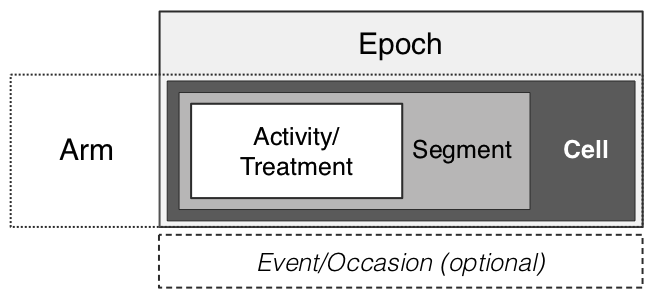
\includegraphics[height=0.2\textheight]{pics/CellSegmentEpochArmEvent_concept}%
 \caption{Overview of the basic concept of the Trial Structure: arm, 
 epoch, event and a cell with segment and activity/treatment as used in the CDISC Study
   Design Model. See the next figure for an example.}
 \label{fig:CellSegmentEpochArmEvent_concept}
 \end{figure}
 \begin{figure}[htb]
 \centering
 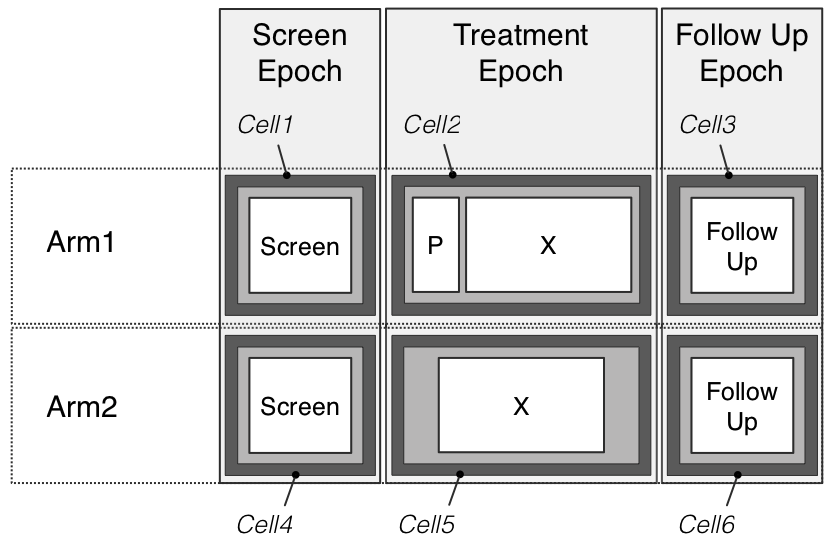
\includegraphics[height=0.35\textheight]{pics/templateTrialDesign}%
 \caption{An example of a study with two arms and three epochs: Screen, 
 Treatment and Follow Up. A segment can contain more then one Activity/Treatment
 as can be seen in the \var{Cell2} with one Pre-treatment \var{P} and Treatment \var{X}.
 In this particular example no Event/Occasion is specified.}
 \label{fig:templateTrialDesign}
 \end{figure}
 Using this design gives us the reassurance that \pharmml will be able
 to represent all trial structures that we are likely to encounter. Figure 
 \ref{fig:templateTrialDesign} shows one such example of an hypothetical trial
 consisting of two arms, three epochs: \var{Screen}, \var{Treatment} and 
 \var{Follow Up}. There are accordingly six cells and segments, each consisting of one
 or two activities. \var{Cell2} has the most complex structure carrying two
 subsequent treatments, Pre-treatment \var{P} and Treatment \var{X}. In this case 
 no Events/Occasions are specified which is an optional element in the 
 proposed design.\\
 Examples of how a trial design is encoded in \pharmml can be found in
 the examples, see chapter \ref{chap:worked-egs}.


%%%%%%%%%%%%%%%%%%%%%%%%%%%%%%%%%%%%%%%%%%%%%%%%%%%%%%%%%%%%%%%%%
\subsection{Population}
\label{subsec:TrialPopulation}

This is second major element of the trial design description where we  
\begin{itemize}
\item
describe the individuals in the study
\item
describe their attributes (such as weight, gender etc)
\item
assign them to an arm of the study but also 
\item
indicate their country or centre membership to define higher levels of variability above the subject level. 
\end{itemize}
We define the possible attributes of all individuals using the \var{IndividualTemplate} block and then map each individual to this template using a \var{Dataset} block.

%\begin{description}
% \item[] 
%
% \item[Epoch] 
%
% \item[Epoch] 
% 
%\end{description}

%%%%%%%%%%%%%%%%%%%%%%%%%%%%%%%%%%%%%%%%%%%%%%%%%%%%%%%%%%%%%%%%%
\subsection{Individual dosing}
\label{subsec:TrialSIndivDosing}

So far, the two last sections on \var{Structure} and \var{Population} described information
which is sufficient to encode e.g. a simulation task. For an estimation task we need to provide 
experimental data for each dosing activity relevant to the particular case. 
With the current structure we can provide individual dosing information for a every dosing activity,
which can very with time, which was defined in the \var{Structure} part, see \ref{subsec:TrialStructure}.

The structure of this part is similar to the that used in \var{Population} in that first 
a table template is defined with all relevant columns, i.e. \var{ID}, \var{TIME} and \var{DOSE},
which is then populated with individual dosing data.


%%%%%%%%%%%%%%%%%%%%%%%%%%%%%%%%%%%%%%%%%%%%%%%%%%%%%%%%%%%%%%%%%
\subsection{PharmML implementation}
\label{subsec:TrialSIndivDosing}

Dependent on the task to be implemented, the information to be stored 
in the Trial Design block will differ. For example an estimation task requires all three 
elements discussed above which in \pharmml have the intuitive names
\xelem{Structure}, \xelem{Population} and \xelem{IndividualDosing}, 
see figure \ref{fig:simEstTasks_trialList}. For a simulation task only the two first are 
sufficient.

  \begin{figure}[htb]
 \centering
 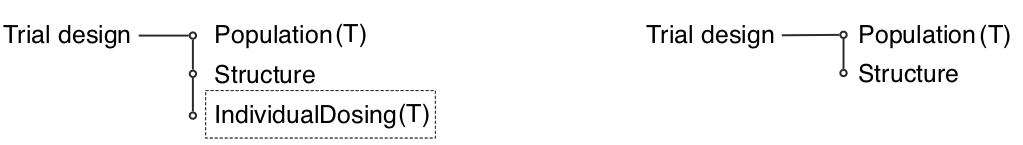
\includegraphics[width=0.7\linewidth]{pics/simEstTasks_trialList}%
 \caption{PharmML building blocks used in the trial definition. (T) indicated that in this
 block a table has to be defined, see chapter \ref{chap:worked-egs} for examples.}
 \label{fig:simEstTasks_trialList}
 \end{figure}




%%%%%%%%%%%%%%%%%%%%%%%%%%%%%%%%%%%%%%%%%%%%%%%%%%%%%%%%%%%%%
%\begin{figure}[htbp!]
%\centering
%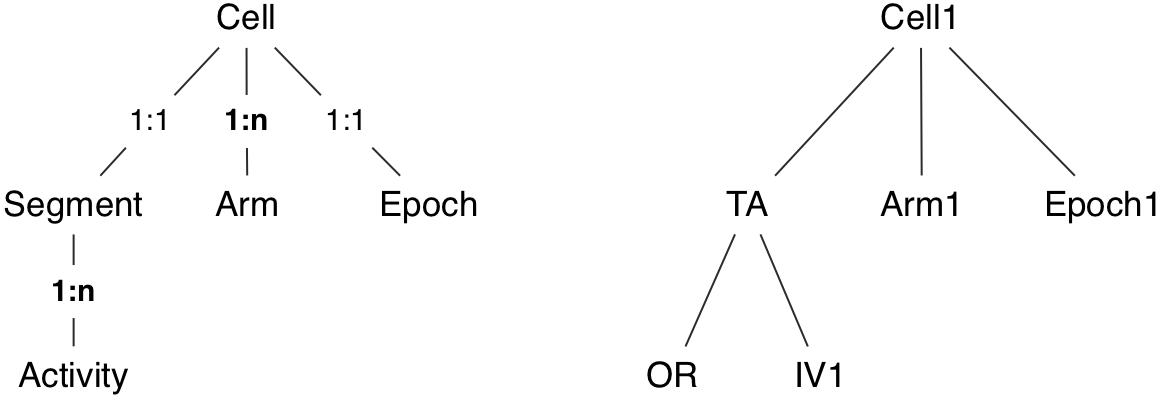
\includegraphics[width=0.8\linewidth]{../pics/cellHierarchy2}
%\caption{General cell hierarchy (left); The root of the hierarchy is the cell which can contain one segment, one epoch and multiple arms. The segment element can have multiple child elements, the activities e.g. treatments or a washout. (right) An example of how it is applied in this example.}
%\label{fig:cellHierarchy}
%\end{figure}

%\section{Design elements and examples}
%\label{sec:CTS_exampleSection} % KEEP THIS LABEL!!!!!!
%The default working mode, as mentioned above, is when all the study characteristics are encoded in the data file. Alternatively, PharmML offers a very flexible structure for the setup of clinical trials. Using only a few basic elements the modeller can compose several types of designs, including parallel design and crossover designs with or without washout or run-in period\footnote{\textit{Run-in} -- do be continued. Definition after \cite{Iverson:2007fk}}, see Figure \ref{fig:CTSfigure1} for examples. The basic elements are:
%
%\begin{itemize}
%\item
%%\textit{Dosing}
%%\begin{itemize}
%%\item
%%one or multiple dosing events can be defined
%%\item
%%dosing type: single dose, sequence/repeated or steady-state dosing
%%\item
%%type of administration: bolus or infusion
%%\item
%%target compartment/variable
%%\item
%%amount and/or infusion rate
%%\item
%%dosing times
%%\end{itemize}
%%\item
%\textit{Treatment} -- describes dosing related data
%\begin{itemize}
%\item
%Administration/dosing type, \textit{Bolus} or \textit{Infusion}, as single value or a sequence
%\item
%Dosing Times -- as single value or a sequence
%\item
%Dose Amount -- as single value or a sequence
%\item
%Dosing target 
%\begin{itemize}
%\item
%Target variable (indicates the target compartment) -- for ODE coded structural models, e.g. $Ad$ the drug amount in the depot compartment (see section \ref{sec:structuralModel})
%\item
%Dose variable -- for explicit algebraic equations with a dose amount variable, e.g. $D$ as in $C(t)= \frac{D}{V}e^{-k(t-t_D)}$
%\end{itemize}
%\end{itemize}
%\item
%\textit{Treatment Epoch\footnote{\textit{Epoch} -- Interval of time in the planned conduct of a study. An epoch is associated with a purpose (e.g., screening, randomization, treatment, follow-up), which applies across all arms of a study. NOTE: Epoch is intended as a standardised term to replace: period, cycle, phase, stage. Definition after \cite{CDICS:2011}}} -- basic time interval within a study
%\begin{itemize}
%\item
%Epoch name, e.g. \textit{Treatment\_A} or \textit{Washout}\footnote{\textit{Washout} -- A period in a clinical study during which subjects receive no treatment for the indication under study and the effects of a previous treatment are eliminated (or assumed to be eliminated).} or \textit{Run-in}
%\item
%\textit{Start time} and \textit{end time} of an epoch -- this sets reference time frame for any possible occasion within an epoch
%\item
%Occasion(s) -- defined by
%\begin{itemize}
%\item
%\textit{start time} and \textit{end time} of each occasion relative to epoch time frame
%\item
%level identifier 
%\end{itemize}
%\end{itemize}
%\item
%\textit{Group} -- basic grouping structure for subjects usually containing one or more treatment epochs
%\begin{itemize}
%\item
%a sequence of epochs for a number of subjects, e.g. [\textit{Epoch\_A}, \textit{Washout}, \textit{Epoch\_B}]
%\item
%number of subjects
%\end{itemize}
%\end{itemize}
%
%\paragraph{Note 1} The name of a particular trial design, e.g. \textit{parallel} or \textit{crossover with washout} is not part of the language. It can be provided as annotation of the trial design model using an appropriate ontology.
%\paragraph{Note 2} The 'Washout' epoch means complete reset of all variables and is defined without start and end times, but this restrictions will be released in an upcoming specification.
%\paragraph{Note 3} The support for variability levels is limited in this specification of PharmML. More specifically, it can only encode occasions definable using start and end times for each occasion. Levels above the subject reference level, such as 'country' or 'centre' cannot be encoded. 
%


%\begin{figure} % [htb!]
%\centering
%\begin{tabular}{c}
% 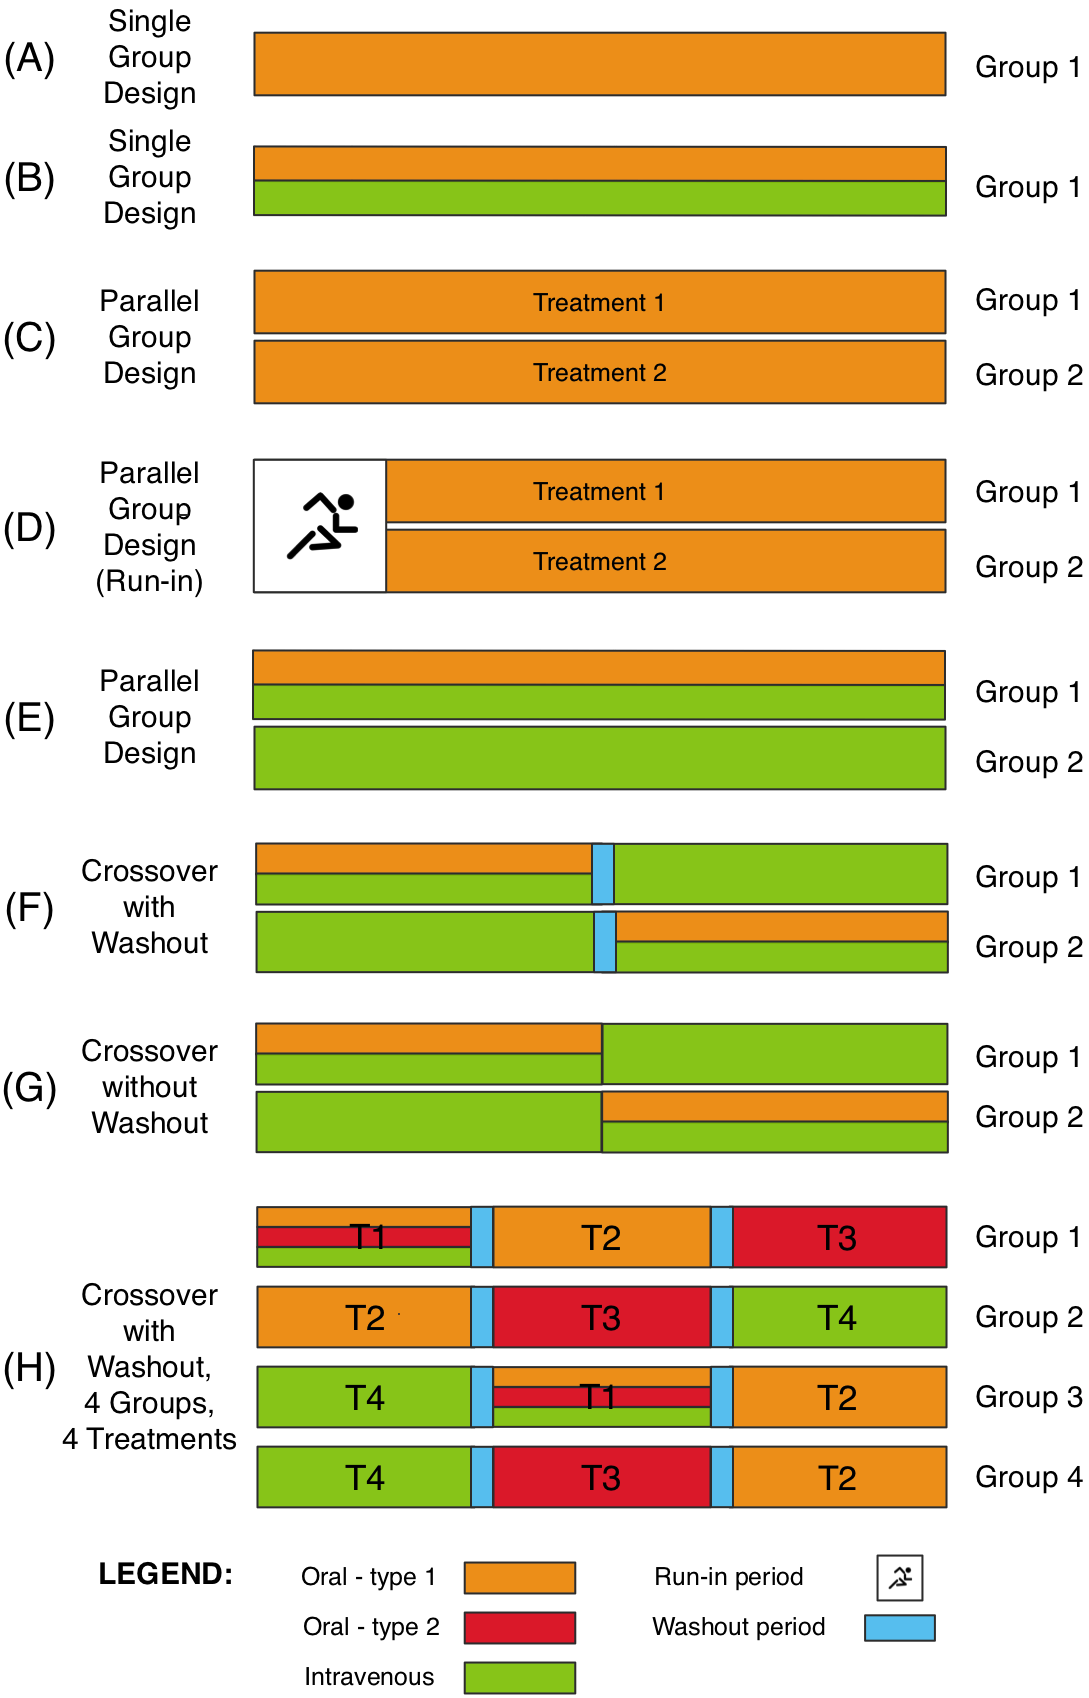
\includegraphics[width=140mm]{ClinicalDesignPatterns_version3}
% \end{tabular}
%\caption{Examples for basic clinical trial design types and configurations. In general any combination of the basic structural elements, i.e. \textit{Dosing}, \textit{Treatment}, \textit{Treatment Epoch} and \textit{Group}, can be created. Based on \cite{Lavielle:2012} and \cite{Wang:2006}.}
%\label{fig:CTSfigure1}
%\end{figure}


%%%%%%%%%%%%%%%%%%%%%%%%%%%%%%%%%%%%%%%%%%%%%%%%%%%%%%%%%%%%%%%%%
%\subsection{Example 1 -- Basic crossover with washout}
%This example describes a crossover design\footnote{\textit{Crossover design} -- Each subject is allocated to a sequence of treatments across a number of treatment periods. Within crossover trials, sequences can include all possible treatments or a subset of these (incomplete block). Definition after \cite{CDICS:2011}} with washout, see example F in Figure \ref{fig:CTSfigure1}.
%
%\subsubsection{Trial design model}
%
%-- Treatment definition
%\begin{align*}
%Treatment\_A: & AdministrationType = \text{[OR bolus, IV bolus]}  \\
%& DoseTime = [6:24:72, 0:24:72]   \\
%& DoseSize = [50, \;\;100]   \\
%& DoseVariable = \text{[D, \;\;D]}  \\
%Treatment\_B: & AdministrationType = \text{OR bolus}  \\
%& DoseTime = 0:24:72   \\
%& DoseSize = 150   \\
%& DoseVariable = \text{D} 
%\end{align*}
%
%-- Treatment Epoch definition
%\begin{align*}
%Epoch\_1: & Treatment\_A  \\
%& TreatmentStart = 0  \\
%& TreatmentEnd = 100  \\
%Epoch\_2: & Treatment\_B  \\
%& TreatmentStart = 0  \\
%& TreatmentEnd = 100  \\
%Epoch\_3: & Washout 
%\end{align*}
%
%-- Group definition
%\begin{align*}
%Group 1: 	& TreatmentSeq = \text{[Epoch\_1, Epoch\_3, Epoch\_2]}	 \\
%			& GroupSize = 40		 \\
%Group 2: 	& TreatmentSeq = \text{[Epoch\_2, Epoch\_3, Epoch\_1]}  \\
%			& GroupSize = 60		
%\end{align*}
%
%
%%%%%%%%%%%%%%%%%%%%%%%%%%%%%%%%%%%%%%%%%%%%%%%%%%%%%%%%%%%%%%%%%
%\subsection{Example 2 -- Complex crossover trial with washout, 4 groups}
%See example H in Figure \ref{fig:CTSfigure1}.
%
%\subsubsection{Trial design model}
%
%-- Treatment definition
%\begin{align*}
%T1: & AdministrationType = \text{[OR1, OR2, IV]}  \\
%& DoseSize = [50 \;\;\;100 \;\;\;100];   \\
%& DoseTime = [6:24:72, 0:24:72, 12:24:72];   \\
%& DoseVariable = \text{[D, \;\;D, \;\;D]}  \\
%T2: & AdministrationType = \text{OR1}  \\
%& DoseSize = 150;   \\
%& DoseTime = [0:24:72];    \\
%& DoseVariable = \text{D}  \\
%T3: & AdministrationType = \text{OR2}  \\
%& DoseSize = 150;   \\
%& DoseTime = [0:24:72];   \\
%& DoseVariable = \text{D}  \\
%T4: & AdministrationType = \text{IV}  \\
%& DoseSize = 150;   \\
%& DoseTime = [0:24:72];   \\
%& DoseVariable = \text{D}  
%\end{align*}
%
%
%-- Treatment Epoch definition
%\begin{align*}
%Epoch\_1: & T1  \\
%& TreatmentStart = 0  \\
%& TreatmentEnd = 100  \\
%Epoch\_2: & T2  \\
%& TreatmentStart = 0  \\
%& TreatmentEnd = 100  \\
%Epoch\_3: & T3  \\
%& TreatmentStart = 0  \\
%& TreatmentEnd = 100  \\
%Epoch\_4: & T4  \\
%& TreatmentStart = 0  \\
%& TreatmentEnd = 100  \\
%Epoch\_5: & Washout 
%\end{align*}
%
%
%-- Group definition
%\begin{align*}
%Group 1: 	& TreatmentSeq = \text{[Epoch\_1, Epoch\_5, Epoch\_2, Epoch\_5, Epoch\_3]}	 \\
%			& GroupSize = 40		 \\
%Group 2: 	& TreatmentSeq = \text{[Epoch\_2, Epoch\_5, Epoch\_3, Epoch\_5, Epoch\_4]}  \\
%			& GroupSize = 40		 \\
%Group 3: 	& TreatmentSeq = \text{[Epoch\_4, Epoch\_5, Epoch\_1, Epoch\_5, Epoch\_2]}	 \\
%			& GroupSize = 60		 \\
%Group 4: 	& TreatmentSeq = \text{[Epoch\_4, Epoch\_5, Epoch\_3, Epoch\_5, Epoch\_2]}  \\
%			& GroupSize = 60		
%\end{align*}





%%%%%%%%%%%%%%%%%%%%%%%%%%%%%%%%%%%%%%%%%%%%%%%%%%%%%%%%%%%%%%%%%
%\subsubsection{To-Do list}
%
%\paragraph{Crossover - other aspects not covered yet}
%- 2x2 -- covered already \\
%- p x q -- see Table 2 in \cite{Wang:2006} \\
%- Latin square 3x3 \& 4x4
%
%
%%%%%%%%%%%%%%%%%%%%%%%%%%%%%%%%%%%%%%%%%%%%%%%%%%%%%%%%%%%%%%%%%
%\paragraph{Factorial design}
%In a factorial design two or more treatments are evaluated simultaneously through the use of varying combinations of the treatments. The simplest example is the 2x2 factorial design in which subjects are randomly allocated to one of the four possible combinations of two treatments, A and B say. These are: A alone; B alone; both A and B; neither A nor B. Source: \cite{EMA:1998}\\
%- no example available
%
%\paragraph{Other aspects of factorial design to be considered}
%- 2x2, Ix J x K, unbalanced, 'complicated'
%
%
%%%%%%%%%%%%%%%%%%%%%%%%%%%%%%%%%%%%%%%%%%%%%%%%%%%%%%%%%%%%%%%%%
%\paragraph{Cohort study} 
%Study of a group of individuals, some of whom are exposed to a variable of interest, in which subjects are followed over time. Cohort studies can be prospective or retrospective. [AMA Manual of Style] See also prospective study.
%
%%%%%%%%%%%%%%%%%%%%%%%%%%%%%%%%%%%%%%%%%%%%%%%%%%%%%%%%%%%%%%%%%
%\paragraph{Prospective study} 
%Investigation in which a group of subjects is recruited and monitored in accordance with criteria described in a protocol.
%
%
%%%%%%%%%%%%%%%%%%%%%%%%%%%%%%%%%%%%%%%%%%%%%%%%%%%%%%%%%%%%%%%%%
%\paragraph{Survival} 
%Observe N subjects until at most time T (censored observations). Alternatively observe N subjects until at least R events occur.\\
%- no example available
%
%
%%%%%%%%%%%%%%%%%%%%%%%%%%%%%%%%%%%%%%%%%%%%%%%%%%%%%%%%%%%%%%%%%
%\paragraph{Observational}
%Subjects are not randomly allocated to treatment.\\
%- no examples available
%
%
%%%%%%%%%%%%%%%%%%%%%%%%%%%%%%%%%%%%%%%%%%%%%%%%%%%%%%%%%%%%%%%%%
%\paragraph{Dose escalation Methods in Phase I, \cite{Le-Tourneau:2009fk}}
%-- Rule-based designs: \\
%Traditional 3+3 design, Accelerated titration designs, Pharmacologically guided dose escalation\\
%Model-based designs: \\
%-- Modified continual reassessment method, Escalation with overdose control, Time-to-event continual reassessment method, EffTox -- efficacy and toxicity method, TriCRM -- an adaptive continual reassessment method that considers three potential trial outcomes: no efficacy and no toxicity, efficacy only, and toxicity only\\
%
%%%%%%%%%%%%%%%%%%%%%%%%%%%%%%%%%%%%%%%%%%%%%%%%%%%%%%%%%%%%%%%%%
%\paragraph{Additional option/criteria -- from Mike's list}
%Within each of these general types of study there are several possible flavours:\\
%Titration, Forced titration, Target concentration, Adaptive, With stopping rules, With interim analyses\\
% - no examples available
%
%%%%%%%%%%%%%%%%%%%%%%%%%%%%%%%%%%%%%%%%%%%%%%%%%%%%%%%%%%%%%%%%%
%\paragraph{Other classification criteria} 
%
%\paragraph{Blinding:}
%open/unblinded, single/double/triple  blinded
%
%\paragraph{Order of study}
%- pxq, IxJxK 





 